% !TeX root = ../dokumentation.tex

\addchap{\langanhang}
\renewcommand{\thefigure}{A\arabic{figure}}

\setcounter{figure}{0}



\begin{lstlisting}[label=list:MQClass, caption={Auswertung der MQ-Sensorwerte}]
import time
import math
from MCP3008 import MCP3008

class MQ():

	# define which analog input channel you are going to use (MCP3008)
	MQ_PIN                       = 0        
	# define the load resistance on the board, in kilo ohms
	RL_VALUE                     = 5        
	# RO_CLEAR_AIR_FACTOR derived from the chart in datasheet
	RO_CLEAN_AIR_FACTOR          = 3.57    
	
	CALIBARAION_SAMPLE_TIMES     = 500       
	CALIBRATION_SAMPLE_INTERVAL  = 100      
	READ_SAMPLE_INTERVAL         = 50       
	READ_SAMPLE_TIMES            = 5        
	
	GAS_CO2                      = 0
	GAS_CO                       = 1
	GAS_NH4                      = 2
	
	def __init__(self, Ro=4, analogPin=0):
	self.Ro = Ro
	self.MQ_PIN = analogPin
	self.adc = MCP3008()
	
	#Sensore specific lien
	self.CO2Curve = [1,0.352,-0.331]   
	self.COCurve = [1,0.462,-0.258]  
	self.NH4Curve =[1,0,423,-0.423]   
	
	print("Calibrating...")
	self.Ro = self.MQCalibration(self.MQ_PIN)
	print("Calibration is done...\n")
	print("Ro=%f kohm" % self.Ro)
	
	
	def MQPercentage(self):
	
		val = {}
		read = self.MQRead(self.MQ_PIN)
		val["CO2"]  = self.MQGetGasPercentage(read/self.Ro, self.GAS_CO2)
		val["CO"]   = self.MQGetGasPercentage(read/self.Ro, self.GAS_CO)
		val["NH4"]  = self.MQGetGasPercentage(read/self.Ro, self.GAS_NH4)
		return val
	
	def MQResistanceCalculation(self, raw_adc):
		if(raw_adc != 0):
		return float(self.RL_VALUE*(1023.0-raw_adc)/float(raw_adc));            
		else:
		return 0.0;
	
	def MQCalibration(self, mq_pin):
		val = 0.0
		count = 0
		for i in range(self.CALIBARAION_SAMPLE_TIMES):          
			helper = self.MQResistanceCalculation(self.adc.read(mq_pin))
			#handle errors		
			if(helper != 0.0):
			val += helper
			count = count +1
			time.sleep(self.CALIBRATION_SAMPLE_INTERVAL/1000.0)
	
		val = val/count                                         
	
		val = val/self.RO_CLEAN_AIR_FACTOR                     
		# according to the chart in the datasheet 
		return val;
	
	
	def MQRead(self, mq_pin):
		rs = 0.0
		
		for i in range(self.READ_SAMPLE_TIMES):
		rs += self.MQResistanceCalculation(self.adc.read(mq_pin))
		time.sleep(self.READ_SAMPLE_INTERVAL/1000.0)
		
		rs = rs/self.READ_SAMPLE_TIMES
		
		return rs
	
	def MQGetGasPercentage(self, rs_ro_ratio, gas_id):
		if ( gas_id == self.GAS_CO2 ):
			return self.MQGetPercentage(rs_ro_ratio, self.CO2Curve)
		elif ( gas_id == self.GAS_CO ):
			return self.MQGetPercentage(rs_ro_ratio, self.COCurve)
		elif ( gas_id == self.GAS_NH4 ):
			return self.MQGetPercentage(rs_ro_ratio, self.NH4Curve)
		return 0

	def MQGetPercentage(self, rs_ro_ratio, pcurve):
		return (math.pow(10,( ((math.log(rs_ro_ratio)-pcurve[1])/ pcurve[2]) + pcurve[0])))
	

\end{lstlisting}
\newpage
\begin{figure}
	\centering
	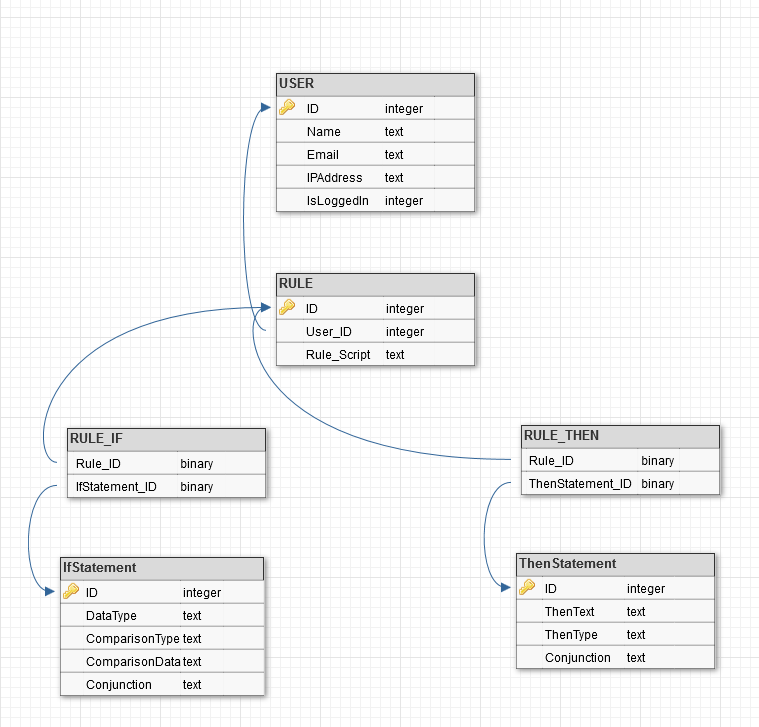
\includegraphics[width=1\textwidth]{images/DBSchema.png}
	\caption{Datenbank Schema der Android SQLite Datenbank}
	\label{fig:androiddbschema}
\end{figure}